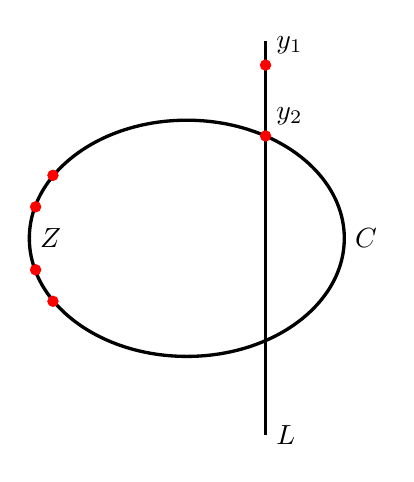
\begin{tikzpicture}[very thick]
  \draw (0,0) ellipse (2 and 1.5) (2,0) node [right] {$C$};
  \draw (1,2.5) -- (1,-2.5) node [right] {$L$};
  \draw[red,fill] (1, 2.2) circle (0.05) node [black, above right] {$y_1$};
  \draw[red, fill] (1, 1.3) circle (0.05) node [black, above right] {$y_2$};
  \draw[red, fill]
  (-1.92,.4) circle (0.05)
  (-1.7,.8) circle (0.05)
  (-1.92,-.4) circle (0.05)
  (-1.7,-.8) circle (0.05);
  \draw (-2,0) node [black, right] {$Z$};
\end{tikzpicture}

%%% Local Variables:
%%% mode: latex
%%% TeX-master: "../main"
%%% End:
